\chapter{Experimentos}\label{cap.experimentos}

A la hora de crear cualquier sistema es necesario hacer múltiples experimentos que nos permitan llegar a ciertas conclusiones que nos sean útiles a la hora de mejorar el diseño. Dichos experimentos deben ser evaluados de alguna forma para comprobar la calidad de los resultados que obtenemos. En este trabajo en concreto se ha recurrido a la herramienta \textit{DetectionSuite}~\cite{detectionsuite} para llevar a cabo dicha evaluación.

Con \textit{DetectionSuite} se obtienen medidas de calidad tales como la precición y el recall medios (\acrshort{map} y \acrshort{mar}) de todas las clases en función de la \acrfull{iou}. En nuestro caso nos hemos quedado con las medidas que tienen un \acrshort{iou} como mínimo de 0.5, pues se ha considerado que es suficiente para medir la calidad.

Este Capítulo vamos a dividirlo en cinco secciones en las cuales hablaremos de lo siguiente:
\begin{itemize}
    \item Evaluación de diversas redes neuronales
    \item Evaluación ampliando Dataset
    \item Evaluación de Darknet con diferentes conjuntos  de imágenes
    \item Evaluación de Smart-Traffic-Sensor
    \item Evaluación de los tiempos de procesamiento
\end{itemize}

A lo largo de este Capítulo se van a ver diferentes experimentos realizados y las medidas obtenidas con ellos en cuanto al \acrfull{map}, \acrfull{mar} con un mínimo de 0.5 \acrshort{iou}, y el tiempo de procesamiento que dedica al realizar las detecciones.

Hay que decir que todos los experimentos realizados con \textit{DetectionSuite} se han hecho desde un ordenador sin GPU, por ello se verá que los tiempos medios de procesamiento son un poco elevados.

\section{Evaluación de diversas redes neuronales}
 
Tal y como se ha comentado en el Capítulo~\ref{cap.diseno} se han realizado pruebas con diferentes \textit{frameworks}. En concreto con \textit{TensorFlow}, \textit{Keras}, y \textit{Darknet}. Para cada plataforma se empleó una red diferente. Con ello se pretendía ver cual era la red que mejores resultados obtenía, además de dotar a \textit{Smart-Traffic-Sensor} de la capacidad de admitir redes entrenadas con diversos \textit{frameworks}.

Para evaluar las redes neuronales se creó una primera base de datos llamada \textit{Dataset STS}, del cual podemos ver información en el Capítulo~\ref{cap.diseno} en la sección~\ref{sec.base_datos}. Con dicho \textit{dataset} se evaluaron las tres redes empleadas.

Tras realizar esta primera evaluación con el fin de determinar cual era la red neuronal que mejor se comportaba, se creó una base de datos de mayor tamaño, denominada \textit{Dataset STS Enriquecido}. Con dicha base de datos se volvió a evaluar la red neuronal que mejores resultados había obtenido en la evaluación inicial (en este caso la red de \acrshort{yolo}).

\subsection{Resultado con Dataset STS}

Tal y como ya se ha comentado, inicialmente se creó una primera base de datos (\textit{Dataset STS}) con el fin de evaluar las tres redes implementadas (cada una con un \textit{framework} diferente). En la Tabla~\ref{tabla_redes_plataformas} se muestra el nombre de cada una de estas redes, asi como la plataforma que se ha empleado en cada caso.

\begin{table}[H] 
\begin{center}
\begin{tabular}{|l|l|}
\hline
Nombre Redes Neuronales & Plataforma de Deep Learning \\ 
\hline \hline
ssd300adam.h5 [\ref{sub.keras}] & Keras \\ \hline
frozen\_inference\_graph.pb [\ref{sub.tensorflow}] & TensorFlow \\ \hline
yolov3\-voc.weights [\ref{sub.darknet}] & Darknet \\ \hline
\end{tabular}
\caption{Redes Implementadas con Diferentes Plataformas}
\label{tabla_redes_plataformas}
\end{center}
\end{table}

Para llevar a cabo el entrenamiento en todas las redes mencionadas se ha empleado el \textit{Dataset STS}, el cual se compone de 3173 imágenes de entrenamiento y 303 imágenes de test. Todas ellas en condiciones meteorológicas favorables y con buena calidad. Las 3173 imágenes de entrenamiento contienen muestras de las diferentes clases (\textit{car, motorcycle, van, bus, truck, small-truck} y \textit{tank-truck}) tal y como se indica en la Tabla~\ref{tabla_database}. En la Tabla~\ref{tabla_datos_primera_evaluacion} se puede ver la cantidad de muestras de cada clase que contienen las 303 imágenes de test.

En el entrenamiento se ha partido de modelos pre-entrenados. Para ver como el entrenamiento con nuestros datos consigue mejorar la capacidad de las redes a la hora de detectar objetos, se han evaluado las redes pre-entrenadas y las entrenadas. La evaluación se ha realizado sobre el conjunto de 303 imágenes de test.

En la Tabla~\ref{tabla_redes_preentrenadas} se pueden ver los resultados obtenidos tras evaluar las redes pre-entrenadas con los datos de test.
\begin{table}[H] 
\begin{center}
\begin{tabular}{|l|l|l|l|}
\hline
Redes Neuronales & mAP & mAR & Mean Inference Time (ms) \\ 
\hline \hline
Keras(VGG\_ILSVRC\_16\_layers\_fc\_reduced.h5) & 0 & 0 & 0\\ \hline
TensorFlow (pre\_frozen\_inference\_graph.pb) & 0.0035 & 0.0373 & 142 \\ \hline
Darknet  (darknet53.conv.74) & 0 & 0 & 14162 \\ \hline
\end{tabular}
\caption{Resultados Redes Pre-Entrenadas}
\label{tabla_redes_preentrenadas}
\end{center}
\end{table}

Los resultados que se obtienen con nuestras redes entrenadas se pueden ver en la Tabla~\ref{tabla_redes_entrenadas}.
\begin{table}[H]
\begin{center}
\begin{tabular}{|l|l|l|l|}
\hline
Redes Neuronales & mAP & mAR & Mean Inference Time (ms) \\ 
\hline \hline
ssd300adam\_inicial.h5 & 0.6709 & 0.7082 & 3194\\ \hline
frozen\_inference\_graph\_inicial.pb  & 0.3283 & 0.4231 & 76 \\ \hline
yolov3\-voc\_inicial.weights  & 0.8641 & 0.9385 & 16894\\ \hline
\end{tabular}
\caption{Resultados Redes Entrenadas}
\label{tabla_redes_entrenadas}
\end{center}
\end{table}

Con toda esta información se puede ver claramente que es necesario re-entrenar las redes con nuestros datos para tener una cierta calidad, ya que cuanto más rico sea el \textit{dataset} con el que se entrena más información podrá adquirir acerca de los objetos a detectar.

Con esta evaluación también se puede ver que los resultados que se obtienen por la red entrenada con \textit{Darknet} son mejores que los de \textit{TensorFlow} y \textit{Keras}. Hay que recordar que con \textit{Darknet} se implementó una red \acrshort{yolo}, con \textit{TensorFlow} una \acrshort{ssd} Mobilenet y con \textit{Keras} una \acrshort{ssd} VGR-16.

Viendo los tiempos de detección se puede ver que cuanto más tiempo tarda la red en realizar la detección mejores resultados obtiene. Esto puede deberse a que la red contiene más capas neuronales o que posee mayor complejidad y por tanto dedica mayor tiempo al procesamiento.


\subsection{Resultados Dataset STS Enriquecido}\label{sec.ampliado_dataset}

Tras la evaluación incial, la primera cuestión que se nos plantea es el enriquecer nuestra base de datos con más imágenes para volver a entrenar la red y ver si sus resultados mejoran. 

La base de datos empleada en este caso para realizar el entrenamiento se llama \textit{Dataset STS enriquecido} y consta de 9774 imágenes. Dicho \textit{dataset} contiene imágenes de buena calidad, de malas condiciones climatológicas y de mala calidad. En este caso para el entrenamiento solo se hizo uso de las imágenes de buena calidad (6717 imágenes de \textit{train}). En la Tabla~\ref{base_datos_final_train} se puede ver la cantidad de esas imágenes de entrenamiento que se emplearon para \textit{train}(5323) y para validación (1394). La Tabla~\ref{tabla_redes_database_mayor} indica la distribución de muestras de las 6717 imágenes de buena calidad.

Con esta nueva base de datos se ha vuelto a realizar el entrenamiento para evaluar como afecta el enriquecimiento de los datos. Además se ha evaluado una red entrenada por Arvind Jayaraman~\cite{CarND_VehicleDetection} para la detección de vehículos con \textit{TensorFlow}. La evaluación se ha vuelto a realizar sobre el conjunto de datos de test de \textit{Database STS} (Tabla~\ref{tabla_datos_primera_evaluacion}). Todos estos datos quedan recogidos en la Tabla~\ref{tabla_redes_entrenadas_mayor_database}

\begin{table}[H]
\begin{center}
\begin{tabular}{|l|l|l|l|}
\hline
Redes Neuronales & mAP & mAR & Mean Inference Time (ms) \\ 
\hline \hline
ssd300adam\_dataset\_enriquecido.h5 & 0.7478 & 0.7831 & 3427\\ \hline
frozen\_inference\_graph\_dataset\_enriquecido.pb  & 0.5484 & 0.61361 & 83 \\ \hline
yolov3\-voc\_dataset\_enriquecido.weights  & 0.9180 & 0.9499 & 15357\\ \hline
Arvind Jayaraman & 0.0384 & 0.0613 & 289\\ \hline
\end{tabular}
\caption{Resultados Redes Entrenadas}
\label{tabla_redes_entrenadas_mayor_database}
\end{center}
\end{table}

Con estos resultados se puede afirmar que el enriquecer la base de datos con mayor información nos da mayor calidad. Además se ha evaluado la red entrenada por Arvind Jayaraman, con lo que se ha visto que se obtienen muy malos resultados.

\subsection{Coste Temporal}

A la hora de realizar el proyecto se ha empleado un ordenador sin GPU y un servidor con GPU. El servidor tiene una tarjeta gráfica GeForce GTX 1080 (Figura~\ref{fig.nvidia}). Y el ordenador una Intel HD Graphics 5500 (Figura~\ref{fig.intel}).

\begin{figure}[H] 
\begin{center}
	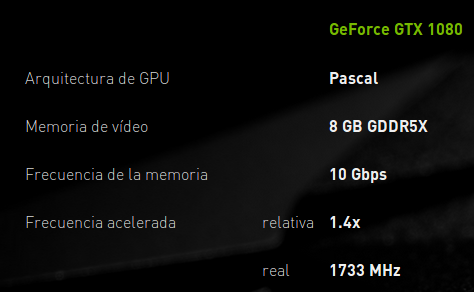
\includegraphics[scale=0.6]{figures/Experimentos/nvidia.png}
   \caption{Características GeForce GTX 1080}
	\label{fig.nvidia}
\end{center}
\end{figure}

\begin{figure}[H] 
\begin{center}
	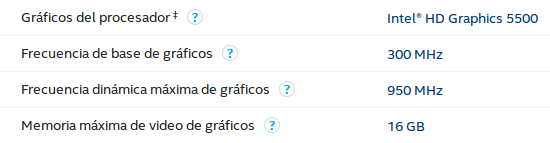
\includegraphics[scale=0.7]{figures/Experimentos/intel.png}
   \caption{Características Intel HD Graphics 5500}
	\label{fig.intel}
\end{center}
\end{figure}

En la Figura~\ref{fig.comparativa} se muestra una comparativa entre ambas tarjetas realizada en la página \textit{UserBenchmark}~\cite{benchmark}, la cual da información acerca de la velocidad que tienen las tarjetas en función a diferentes \textit{benchmark}.

\begin{figure}[H] 
\begin{center}
	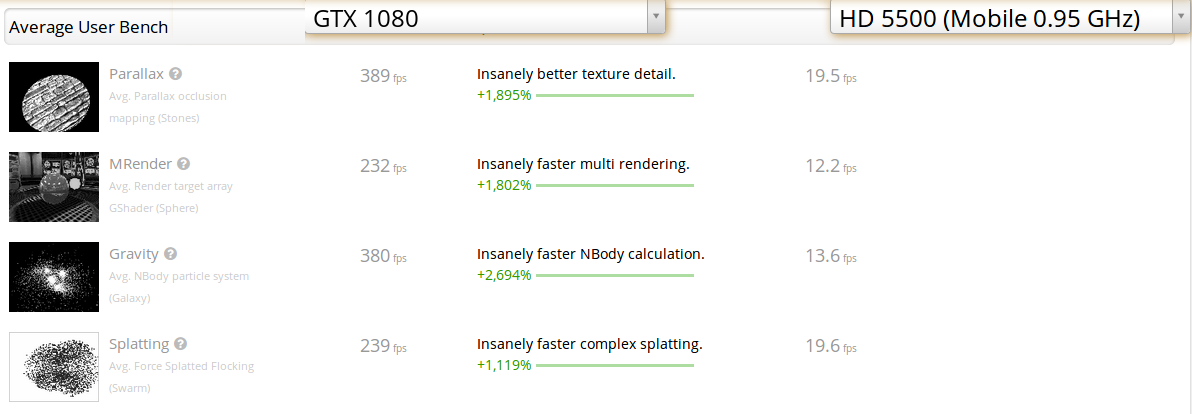
\includegraphics[scale=0.4]{figures/Experimentos/comparativa.png}
   \caption{Comparativa GeForce GTX 1080 y Intel HD Graphics 5500}
	\label{fig.comparativa}
\end{center}
\end{figure}

Todos los experimentos realizados con \textit{DetectionSuite} se han hecho desde el ordenador con la tarjeta gráfica Intel HD 5500 (sin GPU). Para saber si estas redes neuronales tienen un tiempo de procesamiento que nos permita trabajar en tiempo real con un ordenador por supuesto con GPU hemos empleado un servidor. Del cual hemos extraido los resultados con el fin de saber que nuestras redes son capaces de trabajar rápidamente.


En la Tabla~\ref{tiempos} se pueden ver los resultados obtenidos con el servidor y el ordenador sin GPU.

\begin{table}[H]
\begin{center}
\begin{tabular}{|l|l|l|}
\hline
Tipo de Red & Tiempo servidor(ms) & Tiempo ordenador(ms)  \\ 
\hline \hline
Keras & 45 & 3194 \\ \hline
TensorFlow & 19 & 83 \\ \hline
Darknet & 48 & 16894 \\ \hline
\end{tabular}
\caption{Tiempos de procesamiento}
\label{tiempos}
\end{center}
\end{table}

Los resultados que se obtienen respecto a los tiempos de procesamiento con el servidor son bastante razonables y por supuesto permiten trabajar en tiempo real. Tal y como era de esperar el tiempo de procesamiento del ordenador sin GPU es mucho más elevado que el del servidor.

\section{Análisis detallado de la red YOLO}

En este punto ya tenemos identificada cual es la red neuronal que mejores resultados obtiene (\acrshort{yolo}). Es con esta red con la que vamos a continuar haciendo experimentos, es decir, nos hemos centrado en esta red con el fin de mejorar nuestros resultados y llegar a un sistema lo más robusto posible.

Para poder mejorar nuestra red neuronal se ha empleado la base de datos \textit{Dataset STS Enriquecido}, la cual contiene imágenes de buena calidad, de mala calidad y en condiciones meteorológicas desfavorables (lluvia y niebla). En las Figuras~\ref{fig.buena_calidad},~\ref{fig.malas_condiciones} y ~\ref{fig.mala_calidad} se pueden ver ejemplos de dichas imágenes.

\begin{figure}[H] 
\begin{center}
	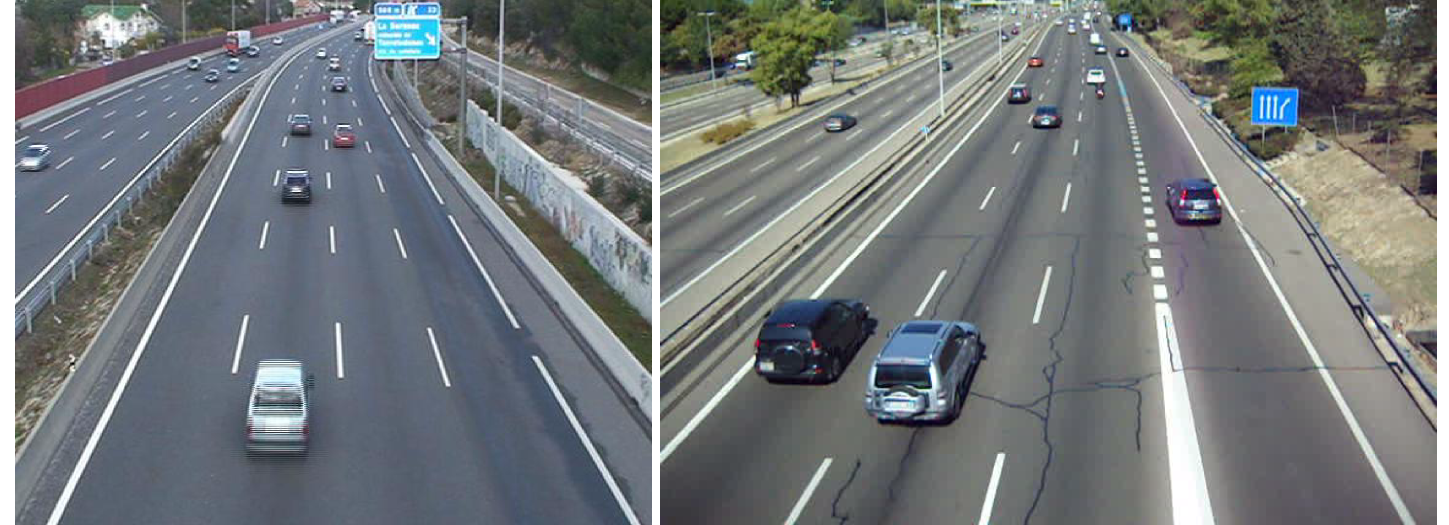
\includegraphics[width=1\textwidth]{figures/Experimentos/buena_calidad.png}
   \caption{Ejemplos de Imágenes de Buena Calidad}
	\label{fig.buena_calidad}
\end{center}
\end{figure}

\begin{figure}[H] 
\begin{center}
	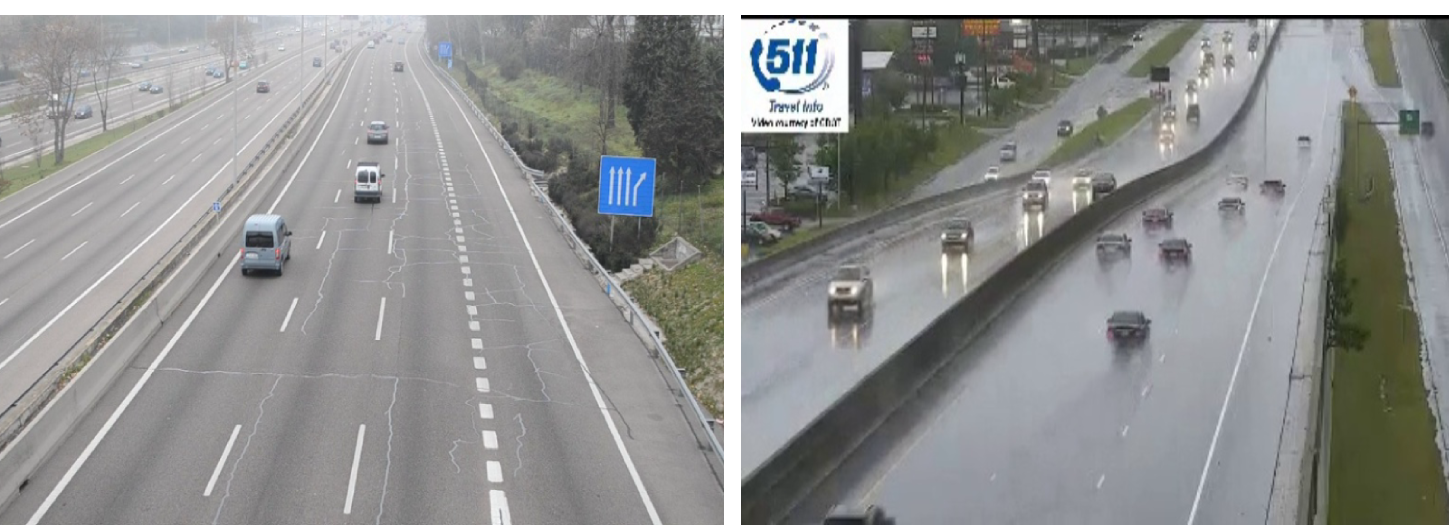
\includegraphics[width=1\textwidth]{figures/Experimentos/malas_condiciones.png}
   \caption{Ejemplos de Imágenes de Malas Condiciones Climatológicas (Niebla y lluvia)}
	\label{fig.malas_condiciones}
\end{center}
\end{figure}

\begin{figure}[H] 
\begin{center}
	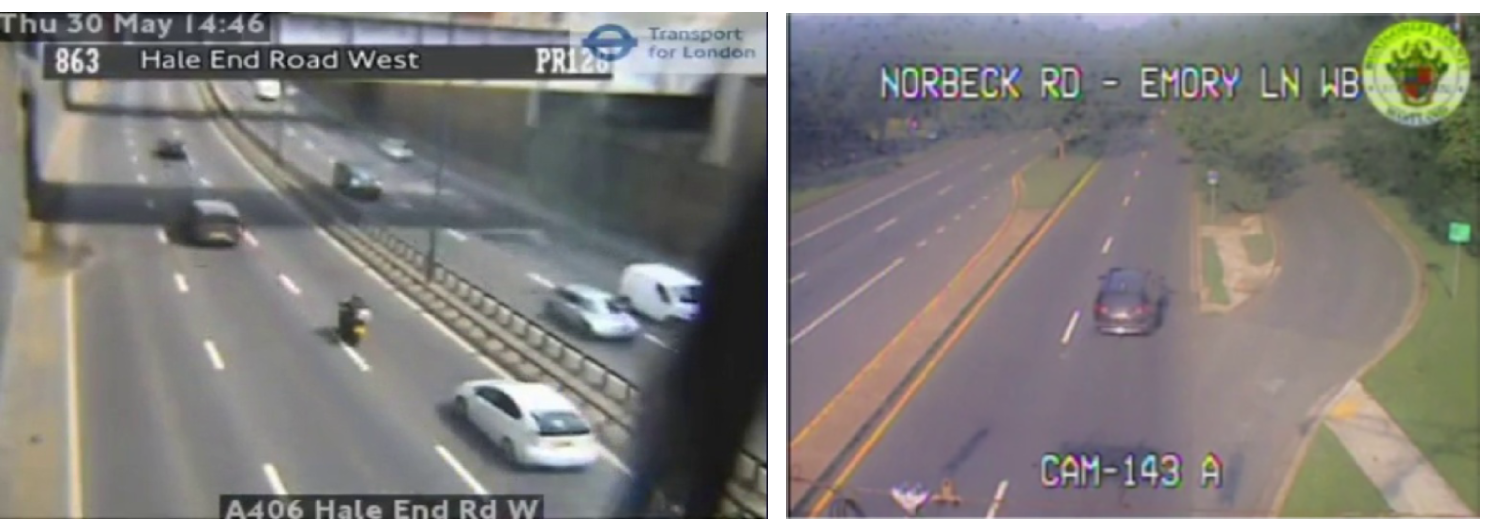
\includegraphics[width=1\textwidth]{figures/Experimentos/mala_calidad.png}
   \caption{Ejemplos de Imágenes de Mala Calidad}
	\label{fig.mala_calidad}
\end{center}
\end{figure}


Para evaluar como afecta el hecho de incorporar imágenes con diferentes condiciones se ha realizado un estudio que engloba 3 etapas:

\begin{enumerate}
    \item En primer lugar se entrenó la red neuronal con imágenes de buena calidad y se evaluó dicha red con  conjuntos de test de imágenes de buena calidad, malas condiciones meteorológicas y mala calidad.
    \item Entrenámos la red neuronal con imágenes de buena calidad y malas condiciones climatológicas. La red resultante la evaluámos con imágenes de buena calidad, malas condiciones meteorológicas y mala calidad.
    \item Finalmente realizamos un entrenamiento con toda la base de datos y lo evaluámos con imágenes de todos los tipos.
\end{enumerate}

\subsection{Buena Calidad}

En un primer lugar tal y como se contaba en la Sección~\ref{sec.ampliado_dataset} se entrenó nuestra red neuronal con un conjunto de un total de 6717 imágenes de buena calidad. Las imágenes de este conjunto incluían información acerca de las diferentes clases que contempla nuestro modelo. Se puede ver en la Tabla~\ref{tabla_redes_database_mayor} la cantidad de muestras de cada clase que contiene este conjunto.

El objetivo de entrenar la red neuronal con solo imágenes de buena calidad es ver como se comporta frente a imágenes de diferentes condiciones. Para ello se ha evaluado este modelo con los 3 tipos de imágenes que tenemos (buena calidad, mala calidad y condiciones desfavorables) por separado y finalmente con un conjunto que incluía imágenes de todos los tipos.

Tras evaluar el modelo entrenado con todos los conjuntos de datos de test (Tabla~\ref{tab_img_test_buenas}, Tabla~\ref{tab_img_test_malas_condiciones} y Tabla~\ref{tab_img_test_mala_calidad}),  se han obtenido los resultados indicados en la Tabla~\ref{resultados_test_buenas}. Hay que decir que se ha evaluado los conjuntos de datos por separado y finalmente se ha hecho una evaluación a un grupo de imágenes de test, a las cuales hemos llamado \textit{Combinado} (incluyen 68 imágenes de cada tipo). Este grupo de imágenes llamado \textit{Combinado} se ve caracterizado en la Tabla~\ref{test_combinado}.

\begin{table}[H] 
\begin{center}
\begin{tabular}{|l|l|l|l|}
\hline
 Conjuntos de Test & Nº de Imágenes & mAP & mAR  \\ 
\hline \hline
Buena Calidad & 389 & 0.9200 & 0.9494 \\ \hline
Malas Condiciones Meteorológicas & 71 & 0.8986 & 0.9379 \\ \hline
Mala Calidad  & 68 & 0.4727 & 0.5470\\ \hline
Combinado & 204 & 0.8311 & 0.8599\\ \hline
\end{tabular}
\caption{Resultados Modelo entrenado con Imágenes de Buena Calidad}
\label{resultados_test_buenas}
\end{center}
\end{table}

\begin{table}[H] 
\begin{center}
\begin{tabular}{|l|l|l|l|}
\hline
Nº de Imágenes  & 204 \\
\hline \hline
Nº de Muestras Totales & 771\\ \hline
Nº Car & 666 \\ \hline
Nº Motorcycle & 7 \\ \hline
Nº Van & 77 \\ \hline
Nº Truck & 5 \\ \hline
Nº Small-Truck & 16 \\ \hline
\end{tabular}
\caption{Conjunto de Test Combinado}
\label{test_combinado}
\end{center}
\end{table}

Observando los resultados se puede comprobar como la red entrenada se comporta perfectamente con las imágenes de buena calidad tal y como era de esperar. Con las imágenes con condiciones meteorológicas desfavorables los resultados también son bastante buenos a pesar de no haber sido entrenada con dichos datos.  Pero en el caso de las imágenes de mala calidad se obtienen resultados muy pobres.

\subsection{Malas Condiciones Meteorológicas}

Tras realizar la evaluación del modelo entrenado con imágenes de buena calidad se procedió a entrenar de nuevo el modelo incluyendo imágenes con condiciones climatológicas malas. Es decir, se ha entrenado el modelo con 6717 imágenes de buena calidad y 1892 imágenes con malas condiciones meteorológicas (Tabla~\ref{tabla_redes_database_malas_condiciones}). Los resultados que se obtienen tras la evaluación pueden comprobarse en la Tabla~\ref{resultados_test_buenas_malas_condiciones}.

\begin{table}[H] 
\begin{center}
\begin{tabular}{|l|l|l|l|}
\hline
 Conjuntos de Test & Nº de Imágenes & mAP & mAR  \\ 
\hline \hline
Buena Calidad & 389 & 0.7759 & 0.8488 \\ \hline
Malas Condiciones Meteorológicas & 71 & 0.9697 & 0.9753 \\ \hline
Mala Calidad  & 68 & 0.6835 & 0.6957\\ \hline
Combinado & 204 & 0.8188 & 0.8442\\ \hline
\end{tabular}
\caption{Resultados Modelo entrenado con Imágenes de Buena Calidad y Condiciones Meteorológicas Malas}
\label{resultados_test_buenas_malas_condiciones}
\end{center}
\end{table}

El hecho de incluir imágenes con condiciones meteorológicas malas hace que el modelo sea capaz de funcionar en mejores condiciones con dicho tipo de imágenes. Además al tener estas imágenes de peor calidad debido a las malas condiciones meteorológicas beneficia al modelo a la hora de detectar vehículos en imágenes de mala calidad. Aunque también afecta a las imágenes de buena calidad, pues la calidad de la detección queda un poco reducida. Si nos fijamos en los resultados con el conjunto total son un pelín inferiores al modelo entrenado únicamente con imágenes de buena calidad, pero son bastante similares.


\subsection{Mala Calidad}

Finalmente se ha entrenado el modelo con toda la base de datos \textit{Database STS Enriquecida}. Esta base de datos tiene las características que se indican en las Tablas~\ref{base_datos_final_train},~\ref{tabla_redes_database_mayor}, ~\ref{tabla_redes_database_malas_condiciones} y ~\ref{tabla_redes_database_mala_calidad}. Los resultados que se obtienen tras la evaluación pueden verse en la Tabla~\ref{resultados_test_todas_img}.

\begin{table}[H] 
\begin{center}
\begin{tabular}{|l|l|l|l|}
\hline
 Conjuntos de Test & Nº de Imágenes & mAP & mAR  \\ 
\hline \hline
Buena Calidad & 389 & 0.7287 & 0.7802 \\ \hline
Malas Condiciones Meteorológicas & 71 & 0.9730 & 0.9779 \\ \hline
Mala Calidad  & 68 & 0.8844 & 0.9010\\ \hline
Combinado & 204 & 0.8606 & 0.8899\\ \hline
\end{tabular}
\caption{Resultados Modelo entrenado con \textit{Dataset STS Enriquecido}}
\label{resultados_test_todas_img}
\end{center}
\end{table}

Al entrenar la red con toda la base de datos los resultados en cuanto a las imágenes de buena calidad quedan algo reducidos de nuevo. Pero en el caso de las imágenes de mala calidad y las de condiciones climatológicas desfavorables los resultados mejoran respecto  a los experimentos anteriores. Consiguiendo así que la evaluación sobre un conjunto de datos de todos los tipos quede mejorada respecto a las pruebas anteriores. 

Con esto se puede ver que cuanto más diversidad tenga la base de datos mayor capacidad tendrá para detectar vehículos en diferentes escenarios. Es decir, enriquecer la base de datos con mayores casos hace que el sistema sea más robusto frente a cambios. 

\section{Comparativa con Traffic-Sensor}

\textit{Smart-Traffic-Sensor} se basa principalmente en \textit{Deep Learning}, pero lo combina con \acrshort{klt} cuando las detecciones realizadas por \textit{Deep Learning} no son suficientes. Esto dota al sistema de mayor robustez. 

El objetivo de este punto es evaluar la calidad del sistema \textit{Smart-Traffic-Sensor} y compararla con el sistema inicial del que se partía (\textit{Traffic-Monitor}~\cite{redo_tesis}). En este sistema la carretera se dividía en una zona de entrada y otra de seguimiento. En la zona de entrada se confirmaba la detección de cada vehículo para posteriormente llevarle un seguimiento.  El sistema de detección que emplea se  basa en la detección del fondo para obtener las detecciones de los vehículos. Una vez pasan estos vehículos a la zona de seguimiento es cuando comienza a clasificarlos y emparejarlos. El seguimiento combina \acrshort{klt} con proximidad espacial al igual que se hace en \textit{Smart-Traffic-Sensor}.

Para la evaluación hemos empleado tres videos con condiciones diferentes (uno con buena calida, otro de lluvia y por último uno de mala calidad). \textit{DetectionSuite} realiza evaluaciones de modelos entrenados sobre un conjunto de datos. En este caso no queremos evaluar el modelo sino el sistema global. Por ello se ha modificado \textit{DetectionSuite} para poder evaluar muestras que se almacenen en un \textit{.txt}. 

En resumen la evaluación del sistema \textit{Smart-Traffic-Sensor} se ha realizado siguiendo los siguientes pasos:

\begin{enumerate}
    \item Se ejecuta \textit{Smart-Traffic-Sensor} con un vídeo y se guardan sus detecciones finales en archivos \textit{.txt}, asi como sus respectivas imágenes.
    \item Nos quedamos con una parte de las detecciones e imágenes obtenidas. Por ejemplo cada 6 imágenes nos quedamos con una. Esto se hace pues sino tendríamos que evaluar una cantidad excesiva de imágenes.
    \item Etiquetamos las imágenes almacenadas con \textit{labelImg}~\cite{labelimg}. Pues necesitamos comparar las detecciones realizadas por \textit{Smart-Traffic-Sensor} con alguna referencia.
    \item Comparamos las detecciones obtenidas por \textit{Smart-Traffic-Sensor} con las etiquetas. Para ello nos hemos apoyado en \textit{DetectionSuite}.
\end{enumerate}


A continuación se muestran los resultados obtenidos para cada video con \textit{Smart-Traffic-Sensor}, \textit{Traffic-Monitor}~\cite{redo_tesis} y empleando únicamente el modelo entrenado.

En primer lugar se evaluó un vídeo de buena calidad, del cual podemos ver en la Figura~\ref{fig.video_buena_calidad} una de las detecciones realizadas por \textit{Smart-Traffic-Sensor}.

\begin{figure}[H] 
\begin{center}
	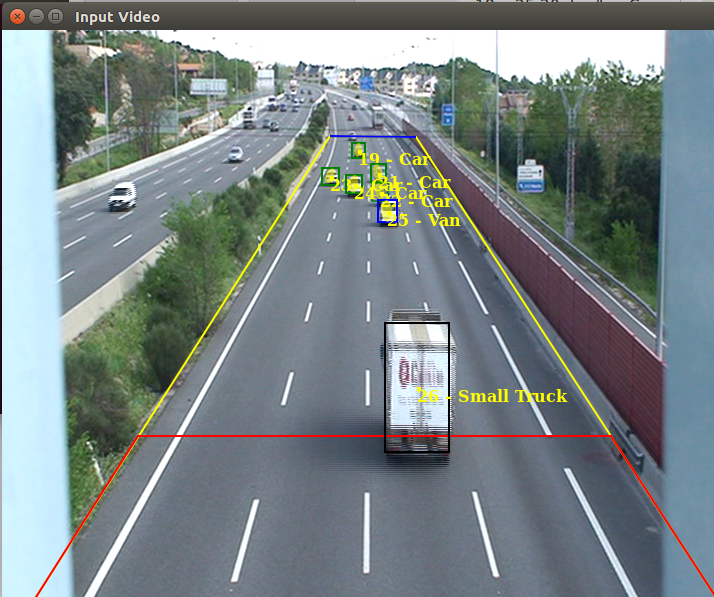
\includegraphics[width=0.7\textwidth]{figures/Experimentos/sts_buena.png}
   \caption{Detecciones Smart-Traffic-Sensor Vídeo Buena Calidad}
	\label{fig.video_buena_calidad}
\end{center}
\end{figure}

De este vídeo se extrajo un total de 299 imágenes que se componen de las muestras que se indican en la Tabla~\ref{tabla_video_bueno}.

\begin{table}[H] 
\begin{center}
\begin{tabular}{|l|l|l|l|}
\hline
Nº de Imágenes  & 299 \\
\hline \hline
Nº de Muestras Totales & 1297\\ \hline
Nº Car & 966 \\ \hline
Nº Motorcycle & 17 \\ \hline
Nº Van & 145 \\ \hline
Nº Truck & 71 \\ \hline
Nº Small-Truck & 98 \\ \hline
\end{tabular}
\caption{Imágenes de Test del Vídeo de Buena Calidad}
\label{tabla_video_bueno}
\end{center}
\end{table}

Los resultados obtenidos con el vídeo de buena calidad se pueden ver en la Tabla~\ref{resultados_video_bueno}. Un vídeo del funcionamiento de \textit{Smart-Traffic-Sensor} se puede ver en \footnote{\url{https://www.youtube.com/watch?v=s0ozbxs0YmY&feature=youtu.be}}.

\begin{table}[H] 
\begin{center}
\begin{tabular}{|l|l|l|l|}
\hline
Tipo de Sistema & mAP & mAR  \\ 
\hline \hline
Smart-Traffic-Sensor & 0.8926 & 0.9009 \\ \hline
Traffic-Monitor & 0.4374 & 0.5940 \\ \hline
Redes Neuronales & 0.8316 & 0.8966\\ \hline
\end{tabular}
\caption{Resultados Vídeo de Buena Calidad}
\label{resultados_video_bueno}
\end{center}
\end{table}

Observando los resultados en esta primera evaluación se puede verificar que el sistema que obtiene mejores resultados es el \textit{Smart-Traffic-Sensor}. El hecho de combinar \acrshort{klt} con las detecciones realizadas mediante \textit{Deep Learning} lo dota de mayor robustez. Esto se hace evidente si nos fijamos en los resultados que se obtienen mediante redes neuronales, con los cuales podemos ver que el hecho de complementarlo con \acrshort{klt} hace que el sistema mejore. No obstante los resultados que se obtienen mediante las redes neuronales son de muy buena calidad, demostrando su gran capacidad a la hora de detectar vehículos. El uso de \acrshort{klt} simplemente lo complementa en casos de oclusiones o vehículos que se vean muy pequeños debido a su lejanía. Por el contrario los resultados que da \textit{Traffic-Monitor} son un poco pobres si los comparamos con los conseguidos gracias a \textit{Smart-Traffic-Sensor}. En las sucesivas pruebas que se han hecho con \textit{Traffic-Monitor} se ha apreciado que no funciona bien con vehículos lejanos (en muchas ocasiones los coches los clasifica como motocicletas) y que en muchas ocasiones tiene dificultad para diferenciar entre coche y furgoneta. Cuando se trata de furgonetas pequeñas las confunde con coches. Esto se debe a que la clasificación se hace mediante modelos 3D, razón por la cual una furgoneta pequeña puede aproximarse más al modelo 3D de un coche que al de una furgoneta grande.


El segundo vídeo que se ha evaluado es un vídeo con condiciones meteorológicas desfavorables. En concreto se trata de un vídeo en condiciones de lluvia. En la Figura~\ref{fig.video_malas_condiciones} se puede ver un ejemplo de \textit{Smart-Traffic-Sensor}.

\begin{figure}[H] 
\begin{center}
	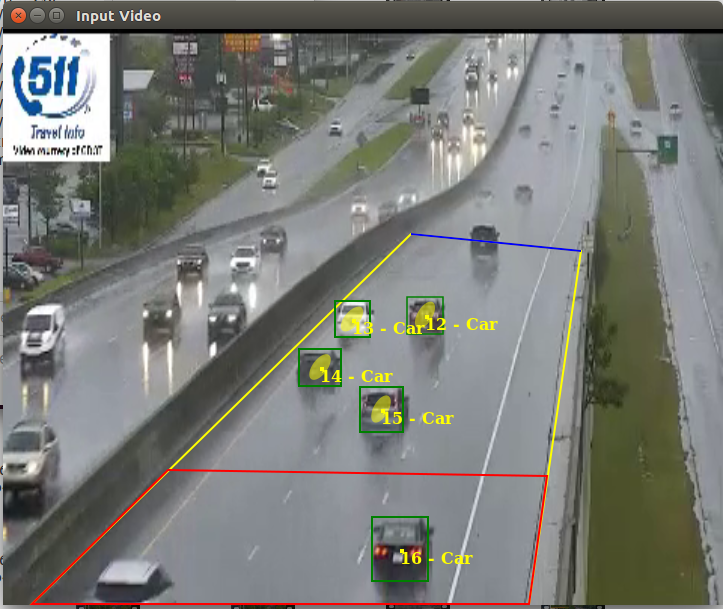
\includegraphics[width=0.7\textwidth]{figures/Experimentos/sts_malas_condiciones.png}
   \caption{Detecciones Smart-Traffic-Sensor Vídeo Malas Condiciones Meteorológicas}
	\label{fig.video_malas_condiciones}
\end{center}
\end{figure}

Con este vídeo se han obtenido 138 imágenes que se componen tan solo de coches tal y como se indica en la Tabla~\ref{tabla_video_malas_condiciones}. Los vídeos que se obtuvieron en condiciones de lluvia no contenían ningún otro tipo de vehículo.

\begin{table}[H] 
\begin{center}
\begin{tabular}{|l|l|l|l|}
\hline
Nº de Imágenes  & 138 \\
\hline \hline
Nº de Muestras Totales & 544\\ \hline
Nº Car & 544 \\ \hline
\end{tabular}
\caption{Imágenes de Test del Vídeo de Malas Condiciones Meteorológicas}
\label{tabla_video_malas_condiciones}
\end{center}
\end{table}

Los resultados obtenidos al evaluar el vídeo de malas condiciones climatológicas se pueden observar en la Tabla~\ref{resultados_video_malas_condiciones}. Podemos ver como se comporta \textit{Smart-Traffic-Sensor} con este vídeo en \footnote{\url{https://www.youtube.com/watch?v=YxpfMtxIr_Q&feature=youtu.be}}.

\begin{table}[H] 
\begin{center}
\begin{tabular}{|l|l|l|l|}
\hline
Tipo de Sistema & mAP & mAR  \\ 
\hline \hline
Smart-Traffic-Sensor & 0.9899 & 0.9926 \\ \hline
Traffic-Monitor & 0.2407 & 0.3162 \\ \hline
Redes Neuronales & 0.9659 & 0.9889\\ \hline
\end{tabular}
\caption{Resultados Vídeo de Malas Condiciones Meteorológicas}
\label{resultados_video_malas_condiciones}
\end{center}
\end{table}

Recapitulando todos los resultados de nuevo se observa que \textit{Smart-Traffic-Sensor} es el sistema que mejores resultados obtiene. A pesar de encontrarnos en condiciones de lluvia es capaz de funcionar y con muy buenos resultados. Con esta prueba se puede ver que \textit{Traffic-Monitor} no es robusto ante cambios, pues no es capaz de funcionar correctamente con lluvia. Esto queda indicado en la tesis que describe \textit{Traffic-Monitor}~\cite{redo_tesis}, en la cual se aclara que la aplicación funciona únicamente con buenas condiciones.

El tercer vídeo que se empleó para evaluar el sistema se trata de un vídeo con mala calidad. En la Figura~\ref{fig.video_mala_calidad} se muestra un ejemplo de dicho vídeo.


\begin{figure}[H] 
\begin{center}
	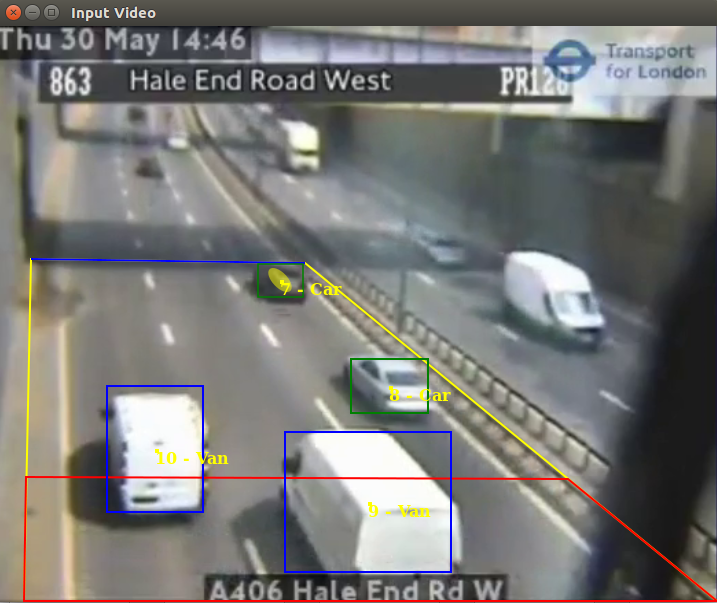
\includegraphics[width=0.7\textwidth]{figures/Experimentos/sts_mala_calidad.png}
   \caption{Detecciones Smart-Traffic-Sensor Vídeo Mala Calidad}
	\label{fig.video_mala_calidad}
\end{center}
\end{figure}

De este vídeo se han obtenido 75 imágenes para poder realizar su evaluación. Estas imágenes se componen de coches, motocicletas y furgonetas tal y como se indica en la Tabla~\ref{tabla_video_mala_calidad}. 

\begin{table}[H] 
\begin{center}
\begin{tabular}{|l|l|l|l|}
\hline
Nº de Imágenes  & 75 \\
\hline \hline
Nº de Muestras Totales & 109\\ \hline
Nº Car & 72 \\ \hline
Nº Motorcycle & 6 \\ \hline
Nº Van & 31 \\ \hline
\end{tabular}
\caption{Imágenes de Test del Vídeo de Mala Calidad}
\label{tabla_video_mala_calidad}
\end{center}
\end{table}

Los resultados obtenidos al evaluar el vídeo de mala calidad se pueden observar en la Tabla~\ref{resultados_video_mala_calidad}. Se puede ver el comportamiento de \textit{Smart-Traffic-Sensor} con este vídeo en \footnote{\url{https://www.youtube.com/watch?v=WZLAyreBNyU&feature=youtu.be}}.

\begin{table}[H] 
\begin{center}
\begin{tabular}{|l|l|l|}
\hline
Tipo de Sistema & mAP & mAR  \\ 
\hline \hline
Smart-Traffic-Sensor & 0.9439 & 0.9444 \\ \hline
Traffic-Monitor & 0.4479 & 0.6303 \\ \hline
Redes Neuronales & 0.9390 & 0.9300\\ \hline
\end{tabular}
\caption{Resultados Vídeo de Mala Calidad}
\label{resultados_video_mala_calidad}
\end{center}
\end{table}

Con toda la información recapitulada se puede decir que \textit{Smart-Traffic-Sensor} es robusto ante imágenes de mala calidad y en condiciones meteorológicas malas. Además es capaz de continuar realizando el seguimiento de los vehículos cuando estos se encuentran muy lejos.
Evidentemente funciona mejor con vehículos próximos, pues es más sencillo detectarlos, pero aún asi es  capaz de detectarlos con gran calidad. Si nos fijamos en los resultados que se obtienen en los tres vídeos se puede comprobar que son mejores para vídeos de mala calidad y condiciones meteorológicas desfavorables que en el caso de buena calidad. Esto tiene su explicación, ya que las exigencias que le marcamos a los datos con buena calidad son mayores. Es decir, en los vídeos de mala calidad y condiciones meteorológicas malas  no esperamos que el sistema sea capaz de detectar vehículos lejanos, pues ni siquiera es sencillo para un ser humano poder clasificar dichos vehículos. Por ello la zona de evaluación que se marca no engloba vehículos que se encuentren muy lejos. A parte de esto, da la casualidad que en estos vídeos la cámara se encuentra a menor distancia de los vehículos que en el caso del vídeo de buena calidad. Esto se hace evidente porque los vehículos que entran en la zona de evaluación tienen mayor tamaño que los que se pueden ver en el vídeo de buena calidad.

Otro detalle es que en el vídeo de buena calidad aparecen más clases de vehículos que en los otros casos, en los cuales la mayoría son coches. La base de datos con la que se ha entrenado la red neuronal posee mayor cantidad de coches que del resto de vehículos, es decir se encuentra desbalanceada. Esto nos lleva a que el modelo llegue a aprender mejor la categoría coche que el resto de categorías. No obstante, se ha apreciado que en todas las categorías se obtienen grandes resultados, exceptuando el caso de las motocicletas. Cuando avanzan los vehículos por la carretera se va reduciendo su tamaño, pues se van alejando. Las motocicletas son vehículos de menor tamaño que el resto de categorías, por ello a nada que avancen empezarán a tomar un tamaño muy reducido, haciendo muy difícil su clasificación. Por esta razón los resultados en cuanto a las motocicletas suelen ser peores a no ser que se encuentren próximos a la cámara y por tanto tengan mayores dimensiones.

Para ver como se comporta el sistema frente a las diversas categorías se han obtenido resultados para cada categoría en el vídeo de buena calidad y en el de mala calidad con \textit{Smart-Traffic-Sensor}. En el de condiciones meteorológicas desfavorable no se ha realizado, pues todos los vehículos que aparecían se correspondían con la categoría coche.

En la Tabla~\ref{resultados_categoria_video_buena_calidad} se pueden ver los resultados que se obtienen con el vídeo de buena calidad y en la Tabla~\ref{resultados_categoria_video_mala_calidad} se pueden apreciar los resultados que nos da el vídeo de mala calidad.

\begin{table}[H] 
\begin{center}
\begin{tabular}{|l|l|l|l|}
\hline
Tipo de Vehículo & mAP & mAR  \\ 
\hline \hline
Car & 0.9457 & 0.9679 \\ \hline
Motorcycle & 0.7029 & 0.7059 \\ \hline
Van & 0.8809 & 0.8897\\ \hline
Truck & 0.9703 & 0.9718\\ \hline
Small-Truck & 0.9604 & 0.9694\\ \hline
\end{tabular}
\caption{Resultados para las Diferentes Categorías en Vídeo de Buena Calidad}
\label{resultados_categoria_video_buena_calidad}
\end{center}
\end{table}

\begin{table}[H] 
\begin{center}
\begin{tabular}{|l|l|l|l|}
\hline
Tipo de Vehículo & mAP & mAR  \\ 
\hline \hline
Car & 1 & 1 \\ \hline
Motorcycle & 0.8317 & 0.8333 \\ \hline
Van & 1 & 1 \\ \hline
\end{tabular}
\caption{Resultados para las Diferentes Categorías en Vídeo de Mala Calidad}
\label{resultados_categoria_video_mala_calidad}
\end{center}
\end{table}

En ambos casos se hace evidente que la categoría motocicleta es la que peores resultados da, debido a su tamaño y por tanto a su complejidad para ser detectada y clasificada.


\section{Comparativa con técnicas del estado del arte}

A continuación vamos a hacer un repaso de los resultados respecto a la detección de vehículos que hemos encontrado en la diferente literatura publicada. Para ver con ello si los resultados que obtenemos son comparables con los que se están publicando.

Y. Abdullah, G. Mehmet, A. Iman and B. Erkan ~\cite{rcnn_detection} propusieron dos soluciones. Una con Faster \acrshort{rcnn} y otra con \acrshort{rcnn}. En su artículo indican el \acrshort{map} obtenido para dos conjuntos de datos tanto con Faster \acrshort{rcnn} como con \acrshort{rcnn}. Esto se puede ver en la Tabla~\ref{resultados_abdullah}.

\begin{table}[H] 
\begin{center}
\begin{tabular}{|l|l|}
\hline
Método & mAP  \\ 
\hline \hline
Faster R-CNN (Dataset 1) & 0.728  \\ \hline
Faster R-CNN (Dataset 2)  & 0.757 \\ \hline
R-CNN (Dataset 1) & 0.647  \\ \hline
R-CNN (Dataset 2)  & 0.657 \\ \hline
Smart-Traffic-Sensor & 0.8926 \\  \hline
\end{tabular}
\caption{Resultados de Y. Abdullah, G. Mehmet, A. Iman and B. Erkan ~\cite{rcnn_detection}}
\label{resultados_abdullah}
\end{center}
\end{table}

L. Chen, F. Ye, Y. Ruan, H. Fan and Q. Chen~\cite{l_chen} usan \textit{k-means} para obtener características de las imágenes y emplearlas durante el entrenamiento. Además concatenan características de diferentes tamaños de imagen. Para realizar la detección emplean \acrshort{cnn}. En la Tabla~\ref{resultados_lchen} se puede ver el \acrshort{map} obtenido con su diseño, asi como los resultados que ha obtenido con otro tipo de redes neuronales.

\begin{table}[H] 
\begin{center}
\begin{tabular}{|l|l|}
\hline
Método & mAP  \\ 
\hline \hline
Fast R-CNN & 0.672  \\ \hline
Faster R-CNN & 0.692 \\ \hline
YOLO & 0.589  \\ \hline
SSD300  & 0.688 \\ \hline
SSD512  & 0.712 \\ \hline
Diseño de L. Chen. et al. & 0.757 \\ \hline
Smart-Traffic-Sensor & 0.8926 \\  \hline
\end{tabular}
\caption{Resultados de L. Chen, F. Ye, Y. Ruan, H. Fan and Q. Chen ~\cite{l_chen}}
\label{resultados_lchen}
\end{center}
\end{table}

Ricardo Guerrero-Gómez-Olmedo, Roberto López-Sastre, Saturnino Maldonado-Bascón and Antonio Fernández-Caballero~\cite{gram-tracking} plantean el uso de filtros de Kalman para realizar el seguimiento y descriptores \acrshort{hog} para la detección y clasificación. En su artículo dicen que la máxima precisión que obtuvieron era de 0.4872.

Albert Soto~\cite{albert_soto} propone el uso de \acrshort{yolo} para la detección de vehículos y llega a obtener una precisión de 0.5893 y un  \textit{recall} de 0.4092.


Viendo todos estos resultados se puede observar que \textit{Smart-Traffic-Sensor} consigue superarlos.Gran parte de esta mejora se debe a la propia arquitectura de red Yolov3, pero otra parte se debe al entrenamiento con la base de datos propia que hemos realizado. En cualquier caso se ha integrado con éxito en la aplicación \textit{Smart-Traffic-Sensor}. Con ello podemos afirmar que hemos llegado a obtener un sistema muy robusto y que aparentemente su calidad es suficientemente buena. Además hemos cumplido con creces el objetivo de mejorar los resultados que ofrecía \textit{Traffic-Monitor}. 